\documentclass[12pt,a4paper]{article}
\usepackage{graphicx}
\usepackage{geometry}
\usepackage{setspace}
\usepackage{hyperref}
\usepackage{titlesec}
\usepackage{fancyhdr}
\usepackage{float}
\usepackage{array}
\usepackage{booktabs}
\usepackage{caption}
\usepackage{lmodern}
\usepackage{amsmath, amssymb}
\usepackage{tikz}
\usetikzlibrary{calc}
\usepackage{longtable}
\usetikzlibrary{positioning, arrows.meta, shapes.geometric}

% Profesyonel listeler için eklendi
\usepackage{enumitem}
\setlist[itemize]{noitemsep, topsep=5pt}
\setlist[enumerate]{noitemsep, topsep=5pt}

\geometry{margin=1in}
\setstretch{1.25}
\captionsetup{font=small, labelfont=bf}

\titleformat{\section}{\normalfont\Large\bfseries}{\thesection.}{0.6em}{}
\titleformat{\subsection}{\normalfont\large\bfseries}{\thesubsection.}{0.6em}{}
\pagestyle{fancy}
\fancyhf{}
\rhead{MycoFlow Project Proposal}
\lhead{Barış Can Ataklı}
\rfoot{\thepage}

\begin{document}

% ==== TITLE PAGE ====
\begin{titlepage}
\centering
{\Huge \bfseries MycoFlow — Bio-Inspired Reflexive QoS System for OpenWrt Routers \par}
\vspace{1.5cm}
{\Large \textbf{Project Proposal Report}\par}
\vspace{2cm}
\textbf{Student:} Barış Can Ataklı\\
\textbf{Advisor:} Dr. Öğr. Üyesi Cihat Çetinkaya\\
\textbf{Department:} Software Engineering, Muğla Sıtkı Koçman University\\
\vfill
{\large November 2025}
\end{titlepage}

\tableofcontents
\newpage

% ==== ABSTRACT ====
\section*{Abstract}
MycoFlow proposes a bio-inspired, fully embedded Quality of Service (QoS) framework for consumer-grade OpenWrt routers.
Taking cues from mycelial networks—which dynamically allocate nutrients and communication pathways based on environmental feedback—MycoFlow implements a reflexive feedback control loop that continuously tunes QoS policies to minimize latency and jitter while preserving fairness and throughput.

The system integrates on-device telemetry (eBPF/netlink) with direct CAKE control; decisions emerge from local sensing and hysteresis-guided reactions rather than machine learning.
The proposed system aims to demonstrate significant latency and jitter reduction compared to static CAKE configurations while maintaining fairness and resource efficiency on constrained hardware.

\textbf{Keywords:} MycoFlow, Bio-Inspired Networking, Adaptive QoS, OpenWrt, CAKE, eBPF, Reflexive Control, Persona-Aware Heuristics, Bufferbloat

\newpage

% ==== INTRODUCTION ====
\section{Introduction and Motivation}
Modern home networks host diverse devices—gaming consoles, smart TVs, PCs, and IoT sensors—all competing for limited bandwidth. Traditional queue management with fixed CAKE parameters fails under changing conditions.
Static QoS policies are unable to account for encrypted traffic, dynamic loads, or heterogeneous device personas.

\subsection*{Motivation}
MycoFlow brings biological adaptivity to router-level QoS.
Mycelial networks excel at local sensing, distributed decision-making, and resource redistribution under stress \cite{fricker2017mycelium,adamatzky2022logics,fukasawa2023foraging}.
MycoFlow translates these principles into network control: each router behaves as a micro-ecosystem that senses, reacts, and stabilizes autonomously.

\section{Problem Statement}
\begin{itemize}
    \item \textbf{Static Configuration:} Fixed queue weights and DSCP policies cannot adapt to congestion.
    \item \textbf{Limited Awareness:} Port or DSCP-based classification fails under QUIC/HTTPS.
    \item \textbf{External Dependencies:} Reliance on remote telemetry reduces efficiency.
    \item \textbf{Poor Observability:} Users lack latency and queue visibility.
\end{itemize}
\textbf{Goal:} Design a self-contained, reflexive, persona-aware QoS system that senses real-time conditions and adjusts CAKE parameters dynamically.

\newpage

% ==== BACKGROUND ====
\section{Background and Related Work}
DiffServ, CoDel, fq\_codel, and CAKE algorithms mitigate bufferbloat through active queue management and fairness.
Recent works extend this baseline:
\begin{itemize}
  \item \textbf{DeepFlow (ACM SIGCOMM 2023):} Lightweight CNN for encrypted traffic classification.
  \item \textbf{Popescu et al. (IEEE Access 2024):} eBPF telemetry maps for adaptive edge metrics.
  \item \textbf{CAKE 2024:} diffserv auto-learning and per-tin delay awareness.
  \item \textbf{LuCI Next (2024):} WebSocket-based real-time dashboards for OpenWrt.
\end{itemize}
MycoFlow departs from ML-heavy designs, focusing on bio-inspired reflexive feedback that adapts locally without cloud intelligence.

\newpage

% ==== BIO-INSPIRED DESIGN ====
\section{Bio-Inspired Design Rationale}
\subsection{Mycelial Principles \& Networking Analogues}
\begin{table}[h]
\centering
\footnotesize
\begin{tabular}{p{4.2cm}p{9.2cm}}
\toprule
\textbf{Mycelial Principle} & \textbf{Networking Analogue in MycoFlow} \\ \midrule
Local sensing of nutrients/stress & eBPF/ICMP/UDP probes measure RTT, jitter, loss, queue depth proxies \\
Adaptive resource translocation & CAKE tin rebalancing, bandwidth caps, DSCP marking updates \\
Hysteresis \& structural stability & Up/Down thresholds, stability timers, gradual parameter ramps \\
Distributed decision-making & Stateless rule evaluation per cycle + state memory for dampening \\
Network remodeling & Periodic refinement of tin shares and persona priorities \\ \bottomrule
\end{tabular}
\caption{Mycelial principles mapped to MycoFlow mechanisms.}
\end{table}

\vspace{0.5cm}

\begin{figure}[H]
\centering
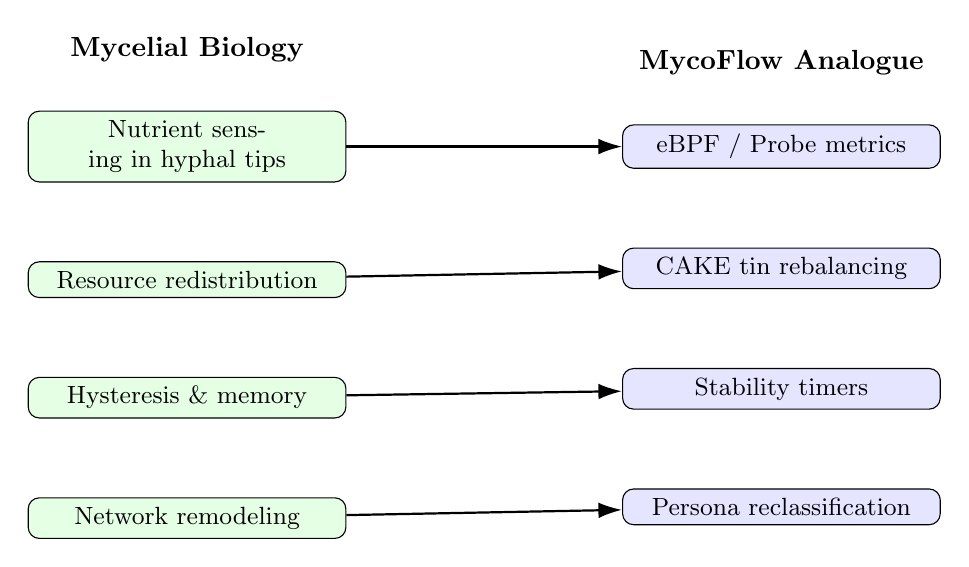
\begin{tikzpicture}[
  every node/.style={align=center, font=\small, text width=3.8cm},
  arrow/.style={-{Latex[length=3mm,width=2mm]}, thick}
]
\node[draw, fill=green!10, rounded corners] (bio1) {Nutrient sensing in hyphal tips};
\node[draw, below=of bio1, fill=green!10, rounded corners] (bio2) {Resource redistribution};
\node[draw, below=of bio2, fill=green!10, rounded corners] (bio3) {Hysteresis \& memory};
\node[draw, below=of bio3, fill=green!10, rounded corners] (bio4) {Network remodeling};

\node[draw, fill=blue!10, rounded corners, right=3.5cm of bio1] (net1) {eBPF / Probe metrics};
\node[draw, below=of net1, fill=blue!10, rounded corners] (net2) {CAKE tin rebalancing};
\node[draw, below=of net2, fill=blue!10, rounded corners] (net3) {Stability timers};
\node[draw, below=of net3, fill=blue!10, rounded corners] (net4) {Persona reclassification};

\draw[arrow] (bio1) -- (net1);
\draw[arrow] (bio2) -- (net2);
\draw[arrow] (bio3) -- (net3);
\draw[arrow] (bio4) -- (net4);

\node[above=0.5cm of bio1, font=\bfseries] {Mycelial Biology};
\node[above=0.5cm of net1, font=\bfseries] {MycoFlow Analogue};
\end{tikzpicture}
\caption{Mapping biological mycelial principles to MycoFlow networking concepts.}
\end{figure}

\newpage

\subsection{Reflexive Control: Formal View}
Let $x_t$ be the metric vector at time $t$ (RTT, jitter, loss, utilization per persona).
The target setpoint is $s$, and the filtered error is
\[
\hat e_t=\alpha e_t+(1-\alpha)\hat e_{t-1}, \qquad e_t=x_t-s.
\]
Control action:
\[
\Delta u_t=
\begin{cases}
+k_u g(\hat e_t), & \hat e_t>\theta_{\text{up}},\\
-k_d g(\hat e_t), & \hat e_t<-\theta_{\text{down}},\\
0,& \text{otherwise.}
\end{cases}
\]
where $g(\cdot)$ is bounded (e.g. $\tanh$) and $(k_u,k_d)$ are rate-limited step gains.

\vspace{1cm}

\begin{figure}[H]
\centering
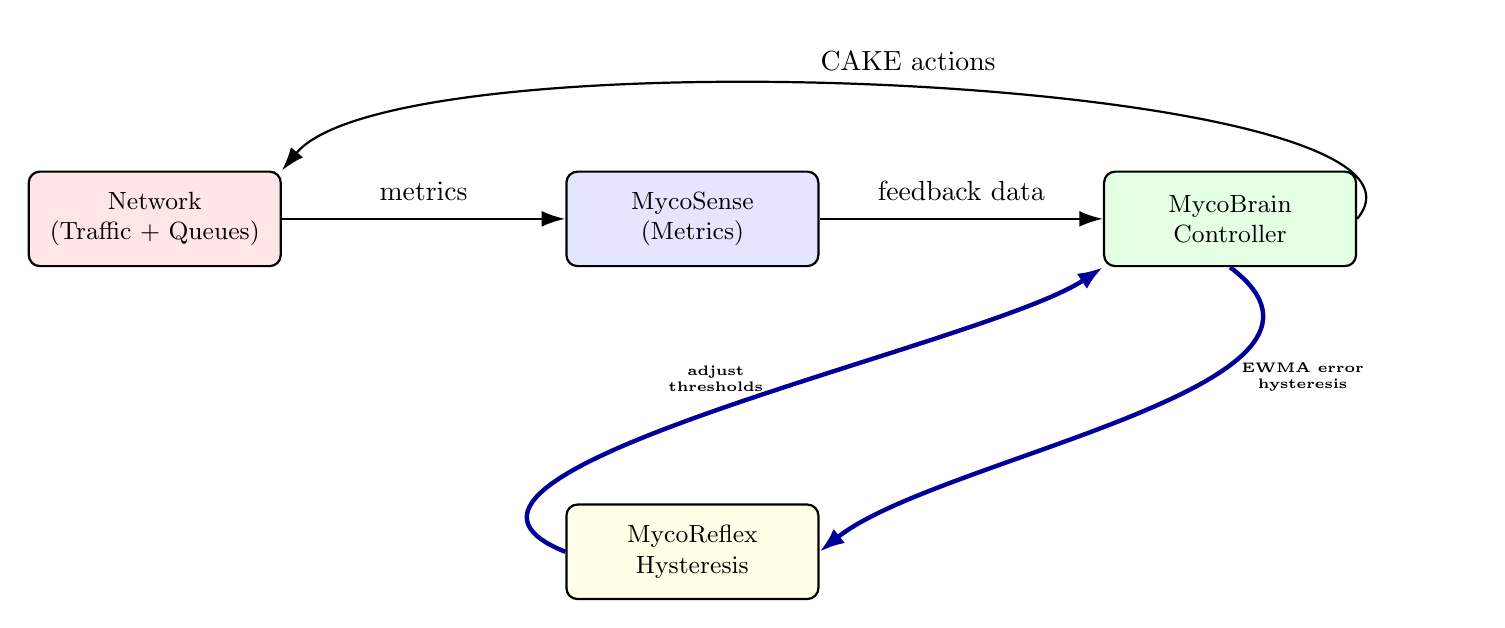
\begin{tikzpicture}[
  node distance=2.2cm and 3.6cm,
  block/.style={draw, thick, rectangle, rounded corners, minimum height=1.2cm, minimum width=3.2cm, align=center, font=\small},
  arrow/.style={-{Latex[length=3mm,width=2mm]}, thick},
  arcarrow/.style={-{Latex[length=3.2mm,width=2.3mm]}, ultra thick, draw=blue!60!black}
]

\node[block, fill=red!10] (network) {Network\\(Traffic + Queues)};
\node[block, right=of network, fill=blue!10] (sense) {MycoSense\\(Metrics)};
\node[block, right=of sense, fill=green!10] (brain) {MycoBrain\\Controller};
\node[block, below=3cm of sense, fill=yellow!10] (reflex) {MycoReflex\\Hysteresis};

\draw[arrow] (network.east) -- node[above, yshift=1mm]{metrics} (sense.west);
\draw[arrow] (sense.east) -- node[above, yshift=1mm]{feedback data} (brain.west);

\draw[arrow]
  (brain.east) .. controls +(1.5,1.8) and +(1.5,1.8) ..
  node[above, yshift=1mm]{CAKE actions}
  (network.north east);

\draw[arcarrow]
  (brain.south) .. controls +(2.0,-1.5) and +(1.5,1.2) ..
  node[pos=0.35, above=2pt, right=1mm, font=\bfseries\tiny, text width=1.8cm, align=center]{EWMA error\\hysteresis}
  (reflex.east);

\draw[arcarrow]
  (reflex.west) .. controls +(-2.5,1.0) and +(-1.5,-1.0) ..
  node[pos=0.6, above=2pt, left=1mm, font=\bfseries\tiny, text width=1.8cm, align=center]{adjust\\thresholds}
  (brain.south west);

\end{tikzpicture}
\caption{Reflexive feedback loop with hysteresis-based control in MycoFlow.}
\end{figure}

\subsection{Persona Inference Heuristics}
The current implementation uses a pragmatic three-signal majority vote for persona classification:
\begin{enumerate}
  \item \textbf{RTT/Jitter signal:} $r_t > 40\text{ms} \lor j_t > 15\text{ms}$ suggests interactive traffic.
  \item \textbf{TX/RX ratio:} $\text{tx\_bps} > 1.5 \cdot \text{rx\_bps}$ indicates bulk upload.
  \item \textbf{Average packet size:} $\bar{s}_t < 200\text{B}$ favors interactive (gaming, VoIP); $\bar{s}_t > 1000\text{B}$ favors bulk.
\end{enumerate}
The final decision is $\arg\max_p \text{vote}_p$ across these signals.
A $k$-of-$m$ sliding window (default $k=3, m=5$) with sticky hysteresis prevents rapid class flips.

\textit{Note: The original design envisioned DNS/SNI categorization and confidence accumulators ($c_p \leftarrow \beta c_p + (1-\beta)\phi_p$). These were simplified to the three-signal heuristic above as a pragmatic compromise for the embedded target, where DNS inspection requires additional kernel hooks.}

\newpage

% ==== SCOPE ====
\section{Scope and Objectives}
\subsection{In-Scope}
\begin{itemize}
\item Embedded packages (\texttt{mycoflowd}, \texttt{luci-app-mycoflow}, \texttt{kmod-myco-ebpf})
\item Reflexive feedback loop with hysteresis and rollback
\item Persona-aware heuristics from DNS + flow features
\item eBPF-backed telemetry with tc/netlink metrics
\item LuCI (Vue-based) dashboard via ubus WebSocket
\end{itemize}

\subsection{Objectives}
\begin{itemize}
\item Reduce median RTT/jitter vs. static CAKE
\item Adaptation $\leq$ 3–5 s
\item CPU $\leq$ 20\%, RAM $\leq$ 64 MB
\item $\geq$ 90\% persona accuracy
\end{itemize}

\newpage

% ==== ARCHITECTURE ====
\section{System Architecture}
\subsection{Reflexive Cycle Diagram (Overview)}

\begin{figure}[H]
\centering
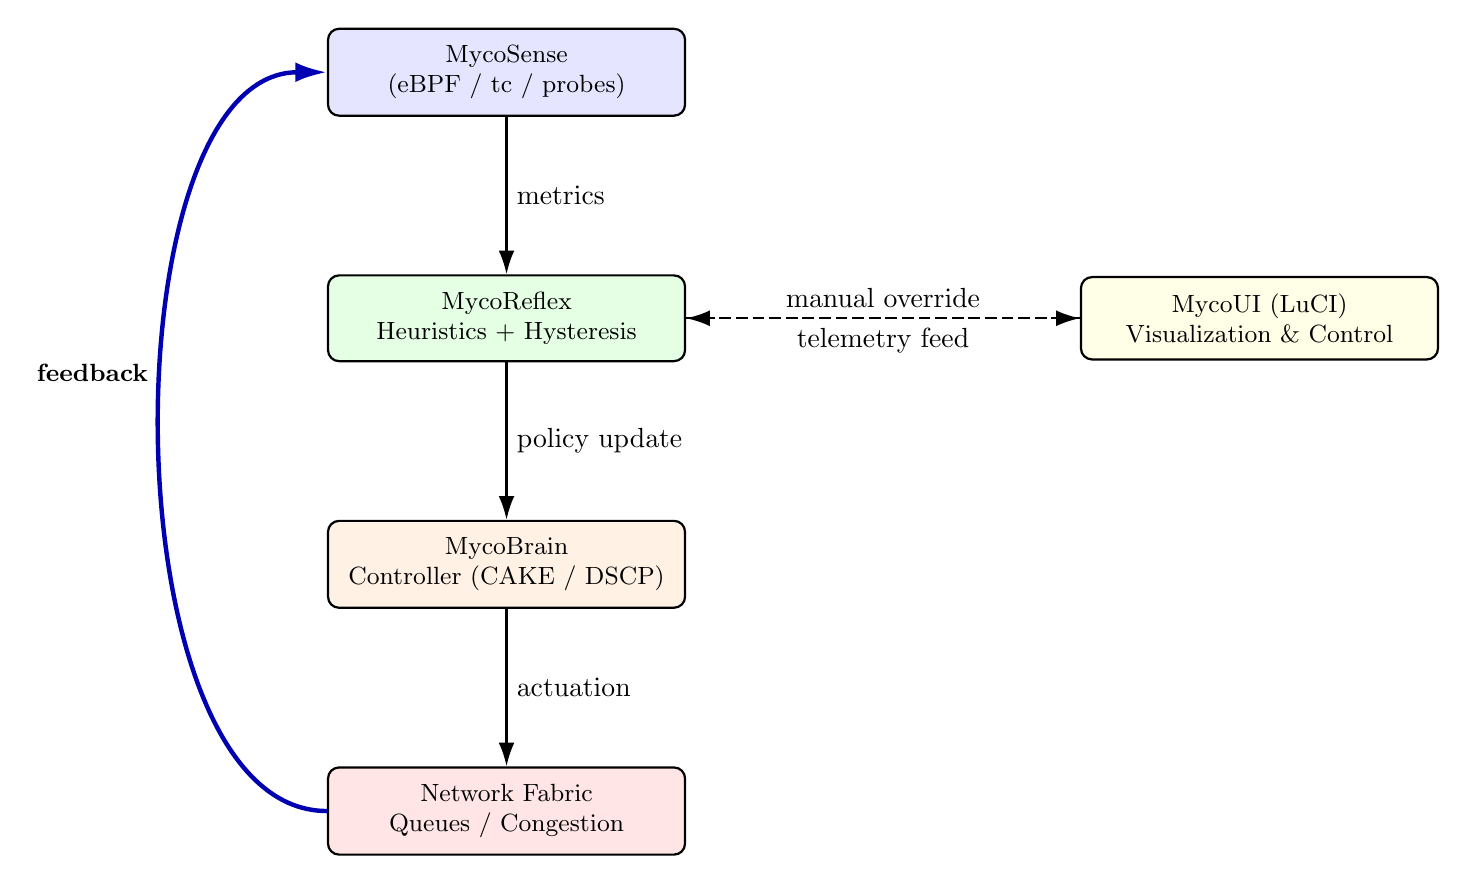
\begin{tikzpicture}[
  node distance=2cm and 2.5cm,
  process/.style={rectangle, rounded corners, draw=black, thick, text width=4.3cm, align=center, inner ysep=6pt, font=\small},
  arrow/.style={-{Latex[length=3mm,width=2mm]}, thick},
  feedbackarrow/.style={-{Latex[length=4mm,width=2.5mm]}, ultra thick, draw=blue!70!black}
]
\node[process, fill=blue!10] (sense) {MycoSense\\(eBPF / tc / probes)};
\node[process, below=of sense, fill=green!10] (reflex) {MycoReflex\\Heuristics + Hysteresis};
\node[process, below=of reflex, fill=orange!10] (brain) {MycoBrain\\Controller (CAKE / DSCP)};
\node[process, below=of brain, fill=red!10] (net) {Network Fabric\\Queues / Congestion};
\node[process, right=5cm of reflex, fill=yellow!10] (ui) {MycoUI (LuCI)\\Visualization \& Control};

\draw[arrow] (sense.south) -- node[right]{metrics} (reflex.north);
\draw[arrow] (reflex.south) -- node[right]{policy update} (brain.north);
\draw[arrow] (brain.south) -- node[right]{actuation} (net.north);

\coordinate (leftmid) at ($(net.west)+(-2.8,0)$);
\coordinate (lefttop) at ($(sense.west)+(-2.8,0)$);
\draw[feedbackarrow]
  (net.west)
  .. controls (leftmid) and (lefttop)
  .. (sense.west)
  node[pos=0.5, xshift=-25pt, yshift=25pt, black, font=\bfseries\small]{feedback};

\draw[arrow,dashed] (ui.west) -- node[above]{manual override} (reflex.east);
\draw[arrow,dashed] (reflex.east) -- node[below]{telemetry feed}(ui.west);
\end{tikzpicture}
\caption{MycoFlow reflexive control cycle from sensing to policy actuation.}
\end{figure}

\newpage

% ==== LIFECYCLE ====
\section{End-to-End Lifecycle}
\subsection{Cold Start \& Bootstrap}
\begin{enumerate}
\item Install packages, enable \texttt{mycoflowd}; set WAN iface and sampling rate.
\item Baseline calibration: brief probe window to estimate idle RTT and variance per tin.
\item Initialize persona priors (optional time-of-day weights).
\end{enumerate}

\subsection{Sense $\rightarrow$ Infer $\rightarrow$ Act $\rightarrow$ Stabilize}
\begin{enumerate}
\item \textbf{Sense:} eBPF/Netlink collect per-flow stats; probes sample RTT/jitter.
\item \textbf{Infer:} Update persona confidences; detect congestion via thresholds on filtered metrics.
\item \textbf{Act:} Apply bounded CAKE/DSCP adjustments with ramping and cooldown timers.
\item \textbf{Stabilize:} If stable for $N$ cycles, decay towards baseline template.
\end{enumerate}

\subsection{Audit, Telemetry, and Rollback}
\begin{itemize}
\item All actions are logged with cause/metric snapshot; a sliding window of states supports rollback.
\item Watchdog detects CPU spikes or metric outliers; freezes loop and reverts to last stable config.
\end{itemize}

\vspace{1cm}

\subsection{Lifecycle Pipeline Diagram}
\begin{figure}[H]
\centering
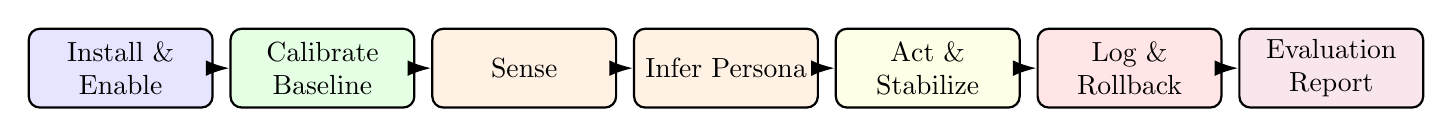
\begin{tikzpicture}[
  node distance=0.2cm, 
  process/.style={draw, thick, rounded corners, minimum height=1cm, 
                  text width=2.1cm, 
                  align=center, fill=blue!10},
  arrow/.style={-{Latex[length=3mm,width=2mm]}, thick}
]
\node[process] (install) {Install \& Enable};
\node[process, right=of install, fill=green!10] (calibrate) {Calibrate Baseline};
\node[process, right=of calibrate, fill=orange!10] (sense2) {Sense};
\node[process, right=of sense2, fill=orange!10] (infer) {Infer Persona};
\node[process, right=of infer, fill=yellow!10] (act) {Act \& Stabilize};
\node[process, right=of act, fill=red!10] (log) {Log \& Rollback};
\node[process, right=of log, fill=purple!10] (report) {Evaluation Report};
\draw[arrow] (install) -- (calibrate);
\draw[arrow] (calibrate) -- (sense2);
\draw[arrow] (sense2) -- (infer);
\draw[arrow] (infer) -- (act);
\draw[arrow] (act) -- (log);
\draw[arrow] (log) -- (report);
\end{tikzpicture}
\caption{End-to-end lifecycle of MycoFlow deployment and operation.}
\end{figure}

\newpage

\section{Implementation Plan and Timeline}

\begin{longtable}{p{2.5cm}p{2cm}p{8.5cm}}
\caption{Six-month implementation roadmap of the MycoFlow project (Nov 2025–May 2026).} \\
\toprule
\textbf{Month / Phase} & \textbf{Duration} & \textbf{Key Deliverables and Tasks} \\
\midrule
\endfirsthead
\toprule
\textbf{Month / Phase} & \textbf{Duration} & \textbf{Key Deliverables and Tasks (continued)} \\
\midrule
\endhead
\midrule
\multicolumn{3}{r}{\textit{Continued on next page}} \\
\bottomrule
\endfoot
\bottomrule
\endlastfoot

\textbf{Month 1 (Nov 2025)} & Weeks 1–4 &
\begin{itemize}[leftmargin=*]
  \item OpenWrt installation on Xiaomi AX3000T; SSH/SCP access validation.
  \item Buildroot toolchain and GitHub repo setup.
  \item Literature review on CAKE, SQM, and bio-inspired networking.
  \item Baseline latency/jitter tests via \texttt{flent} and \texttt{iperf3}.
\end{itemize}
\textbf{Deliverables:} Working router, baseline dataset, CAKE analysis notes. \\

\midrule
\textbf{Month 2 (Dec 2025)} & Weeks 5–8 &
\begin{itemize}[leftmargin=*]
  \item Develop \texttt{mycoflowd} daemon (UCI + ubus integration).
  \item Implement CAKE parameter control via \texttt{tc}.
  \item Add initial metrics collector (RTT, backlog, drops).
\end{itemize}
\textbf{Deliverables:} mycoflowd binary, init script, CAKE control library. \\

\midrule
\textbf{Month 3 (Jan 2026)} & Weeks 9–12 &
\begin{itemize}[leftmargin=*]
  \item Implement feedback control loop (RTT-based adjustment).
  \item Introduce hysteresis with dual thresholds and $k$-of-$m$ voting.
  \item Add rollback and safe-mode logic.
\end{itemize}
\textbf{Deliverables:} Reflexive controller, hysteresis module, rollback system. \\

\midrule
\textbf{Month 4 (Feb 2026)} & Weeks 13–16 &
\begin{itemize}[leftmargin=*]
  \item Integrate eBPF flow tracker (libbpf + TC hook).
  \item Add Netlink statistics and real-time queue metrics.
  \item Enhance probes with jitter/loss tracking.
\end{itemize}
\textbf{Deliverables:} eBPF program, Netlink wrapper, advanced telemetry dataset. \\

\midrule
\textbf{Month 5 (Mar 2026)} & Weeks 17–20 &
\begin{itemize}[leftmargin=*]
  \item Develop \texttt{luci-app-mycoflow} dashboard (WebSocket metrics).
  \item Implement optional persona inference (DNS + flow features).
  \item Conduct end-to-end stress and memory tests.
\end{itemize}
\textbf{Deliverables:} LuCI app, persona engine (optional), full integration test suite. \\

\midrule
\textbf{Month 6 (Apr 2026)} & Weeks 21–24 &
\begin{itemize}[leftmargin=*]
  \item Perform benchmark tests (gaming, conferencing, mixed load).
  \item Tune controller parameters ($\alpha$, cooldown, thresholds).
  \item Statistical analysis and visualization of results.
\end{itemize}
\textbf{Deliverables:} Evaluation dataset, tuning guide, final performance report. \\

\midrule
\textbf{Month 7 (May 2026)} & Weeks 25–26 &
\begin{itemize}[leftmargin=*]
  \item Write final thesis and prepare presentation slides.
  \item Package release and public repository documentation.
\end{itemize}
\textbf{Deliverables:} Final PDF report, LuCI screenshots, release package. \\

\end{longtable}



\vspace{1cm}

% ==== ALGORITHMS ====
\section{Algorithms and Complexity}
\subsection{Congestion Detection}
Let $r_t$ be RTT EWMA and $j_t$ jitter EWMA. Congestion if:
\[
r_t > r_\text{idle} + \delta_r \quad \lor \quad j_t > j_\text{idle} + \delta_j
\]
with tunable margins $(\delta_r,\delta_j)$; debounce via $k$-of-$m$ exceedance.

\subsection{Actuation Scheduling}
Priority queue of pending adjustments with max rate $\rho$ (ops/s) and min gap $\tau_\text{cooldown}$.
Time complexity per cycle $O(F + \log A)$, where $F$ = active flows read from eBPF maps, $A$ = actions.

\subsection{Resource Budget}
\begin{itemize}
\item CPU: target $<20\%$ avg; eBPF sampling at 1–2 Hz; user space loop at 1 Hz.
\item RAM: $<64$ MB including flow tables; cap maps by LRU evict (256-entry userspace flow table).
\item Flash: package $<8$ MB; logs rotated (size/time).
\end{itemize}

\subsection{Implementation Status}
The following modules have been implemented and verified:
\begin{itemize}
  \item \textbf{Modular architecture:} 11 source files (\texttt{main.c}, \texttt{myco\_sense.c}, \texttt{myco\_persona.c}, \texttt{myco\_control.c}, \texttt{myco\_act.c}, \texttt{myco\_ewma.c}, \texttt{myco\_ebpf.c}, \texttt{myco\_netlink.c}, \texttt{myco\_flow.c}, \texttt{myco\_config.c}, \texttt{myco\_log.c}).
  \item \textbf{EWMA filter:} Configurable $\alpha$ applied to RTT and jitter metrics.
  \item \textbf{Thread safety:} Mutex-protected shared state between main loop and ubus thread.
  \item \textbf{eBPF telemetry:} BPF program (\texttt{mycoflow.bpf.c}) with TC hook counting packets/bytes via \texttt{BPF\_MAP\_TYPE\_ARRAY}.
  \item \textbf{Netlink stats:} Raw \texttt{NETLINK\_ROUTE} socket reading Qdisc backlog, drops, and overlimits.
  \item \textbf{Flow table:} Userspace LRU hash table (FNV-1a) populated from \texttt{/proc/net/nf\_conntrack}.
  \item \textbf{Unit tests:} 4 test suites (EWMA, control, config, persona) via CTest.
  \item \textbf{Integration harness:} Docker-based automated test script (\texttt{scripts/run\_integration.sh}).
  \item \textbf{Benchmark suite:} \texttt{iperf3}/\texttt{flent} comparison scripts with JSON output.
\end{itemize}

\newpage

% ==== EVALUATION ====
\section{Evaluation Methodology}
Evaluation uses \texttt{flent} and \texttt{iperf3} under scripted mixed-load profiles.
Each test lasts $\geq 10$ minutes with $\geq 5$ repetitions for statistical confidence (t-test/ANOVA).

\textbf{Scenarios:} Gaming, video conferencing, mixed load, adaptive stress.

\textbf{Metrics:} RTT, jitter, Jain fairness, CPU/RAM.

\textbf{Baselines:} FIFO (no QoS), SQM/CAKE static, qosify, commercial router.

\textbf{Expected:} 40–70\% latency reduction; jitter $<$ 15 ms; fairness $\geq$ 0.9.

\vspace{1cm}

% ==== HARDWARE ====
\section{Hardware Target}
Xiaomi AX3000T (MT7981B, 256 MB RAM).
\begin{itemize}
    \item CPU usage $<$ 20\% avg (40\% peak)
    \item RAM $<$ 64 MB total
    \item Latency overhead $<$ 2 ms
    \item Package size $<$ 8 MB
\end{itemize}

\vspace{1cm}

% ==== SECURITY ====
\section{Security and Ethics}
\begin{itemize}
    \item No payload inspection, only metadata.
    \item No external telemetry by default.
    \item Signed packages, rate-limited ubus calls; least-privilege ubus methods.
\end{itemize}

\newpage

% ==== REPRO ====
\section{Reproducibility and Deployment}
\subsection{Minimal UCI}
\begin{verbatim}
config mycoflow 'core'
  option enabled '1'
  option egress_iface 'pppoe-wan'
  option sample_hz '2'
  option max_cpu '40'
\end{verbatim}

\subsection{ubus Surface}
\begin{verbatim}
myco.status    -> {policy, tins, latency}
myco.persona   -> list|add|delete
myco.policy    -> get|set|boost|throttle
\end{verbatim}

\subsection{Step-by-step}
\begin{enumerate}
\item Install and enable packages; set WAN iface; reboot.
\item Verify eBPF maps and tc stats; run sanity probes.
\item Start traffic profiles; watch LuCI dashboard; collect logs.
\item Export CSV/JSON for analysis; compare against baselines.
\end{enumerate}

\newpage

% ==== FUTURE WORK ====
\section{Future Work}
\begin{itemize}
    \item Cooperative adaptation: routers exchange ``nutrient maps'' (aggregated telemetry).
    \item Optional TinyML persona prediction under strict budgets.
    \item SDN integration via controller APIs for policy orchestration.
    \item Context-aware predictive scheduling (time/location/user mode).
\end{itemize}

\vspace{1.5cm}

% ==== CONCLUSION ====
\section{Conclusion}
Bufferbloat arises from delayed feedback. MycoFlow shortens this delay through reflexive adaptation—sensing queue buildup early and adjusting CAKE weights preemptively.
Each feedback cycle operates at 1 Hz, achieving sub-second reaction time.
Bio-inspired by mycelial networks, MycoFlow redistributes bandwidth like nutrients—sustaining the digital ecosystem without external dependencies.

\newpage

% ==== REFERENCES ====
\begin{thebibliography}{9}
\bibitem{zhao2023} H. Zhao et al., "DeepFlow: Lightweight Deep Learning for Encrypted Traffic Classification," Proc. ACM SIGCOMM, 2023.
\bibitem{popescu2024} M. Popescu et al., "eBPF for Adaptive Network Telemetry on Edge Routers," IEEE Access, 2024.
\bibitem{nichols2024} J. Nichols et al., "CAKE Enhancements for Diffserv Auto-Learning," IETF Draft, 2024.
\bibitem{tang2024} C. Tang and L. Yu, "SDN-Enabled QoS Optimization for Home Networks," IEEE ICC, 2024.
\bibitem{luci2024} OpenWrt GSOC, "LuCI Next: A Modern Web Interface for OpenWrt," 2024.
\bibitem{fricker2017mycelium} M.D. Fricker, L.L.M. Heaton, N.S. Jones, L. Boddy, "The Mycelium as a Network," Microbiology Spectrum, 2017.
\bibitem{adamatzky2022logics} A. Adamatzky, P. Ayres, A.E. Beasley, N. Roberts, M. Tegelaar, M.-A. Tsompanas, H.A.B. Wösten, "Logics in Fungal Mycelium Networks," Logica Universalis, 2022.
\bibitem{fukasawa2023foraging} Y. Fukasawa, M. Savoury, L. Boddy, "Foraging strategies of fungal mycelial networks: responses to resource heterogeneity," Frontiers in Cell and Developmental Biology, 2023.
\end{thebibliography}

\end{document}